\documentclass[a4paper,12pt]{scrbook}

\usepackage{mystyle}
\usepackage{subfiles}

\begin{document}

%\maketitle
\begin{titlepage}
   \vspace*{\stretch{1.0}}
   \begin{center}
     \Huge\textbf{Notes on Higher Categories}\\
     \Large(Work in progress) \\
     \vspace*{1em}
     \Large\textit{Angus Rush}
   \end{center}
   \vspace*{\stretch{1.0}}
   \begin{equation*}
     \begin{aligned}
       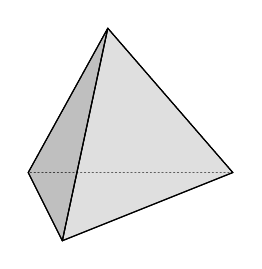
\begin{tikzpicture}[line join = round, scale=1.5, line cap = round]
         \coordinate (3) at (0,{sqrt(2)},0);
         \coordinate (2) at ({-.5*sqrt(3)},0,-.5);
         \coordinate (1) at (0,0,1);
         \coordinate (0) at ({.5*sqrt(3)},0,-.5);

         \draw[densely dotted,] (0)--(2);
         \draw[fill=lightgray,fill opacity=.5] (1)--(0)--(3)--cycle;
         \draw[fill=gray,fill opacity=.5] (2)--(1)--(3)--cycle;
         \draw (1)--(0);
         \draw (1)--(2);
         \draw (2)--(3);
         \draw (1)--(3);
         \draw (0)--(3);
       \end{tikzpicture}
     \end{aligned}
     \qquad\qquad
     \begin{aligned}
       \begin{tikzpicture}[dot/.style={draw,circle,minimum size=1mm,inner sep=0pt,outer sep=0pt,fill=black}, line join = round, scale=1.5, line cap = round]

         \coordinate[draw, dot] (3) at (0,{sqrt(2)},0);
         \coordinate[draw, dot] (2) at ({.5*sqrt(3)},0,-.5);
         \coordinate[draw, dot] (1) at (0,0,1);
         \coordinate[draw, dot] (0) at ({-.5*sqrt(3)},0,-.5);

         \begin{scope}[decoration={markings,mark=at position 0.5 with {\arrow{to}}}]
           \draw[postaction={decorate}] (0)--(1);
           \draw[postaction={decorate}] (0)--(2);
           \draw[postaction={decorate}] (0)--(3);
           \draw[postaction={decorate}] (1)--(2);
           \draw[postaction={decorate}] (1)--(3);
           \draw[postaction={decorate}] (2)--(3);
         \end{scope}
       \end{tikzpicture}
     \end{aligned}
     \qquad \qquad
     \begin{aligned}
       \begin{tikzcd}[row sep=tiny, column sep=tiny]
         && 2
         \arrow[drr]
         \\[2.5em]
         0
         \arrow[urr]
         \arrow[dr]
         \arrow[rrrr]
         &[5em]&&& 3
         \\[0.6em]
         & 1
         \arrow[urrr]
         \arrow[uur, crossing over]
       \end{tikzcd}
     \end{aligned}
   \end{equation*}
   \vspace*{\stretch{0.3}}
\end{titlepage}
\tableofcontents

\subfile{intro.tex}
\subfile{ssets.tex}
\subfile{lifting.tex}
\subfile{homotopy.tex}
\subfile{model.tex}
\subfile{infinity.tex}
\subfile{grothendieck.tex}
\begin{appendices}
  \subfile{cats.tex}
\end{appendices}

\end{document}
